\section{局部二次模型}
\label{sec:sqp-local-model}

站在当前点$\bm{x}^{(t)}$，怎样写出一个既能求解、又能代表原问题的局部模型？一般的问题写成
\begin{equation}
 \begin{aligned}
 \min_{\bm{x}\in\mathbb{R}^n}\quad & f(\bm{x})\\
 \text{s.t.}\quad & g_i(\bm{x})\leq0,\quad i=1,\ldots,m,\\
 & h_j(\bm{x})=0,\quad j=1,\ldots,p,
 \end{aligned}
 \label{eq:sqp-nlp}
\end{equation}
其中$f,g_i,h_j$都二阶连续可微。

\paragraph{约束怎样近似}
Newton法把目标近似到二阶。约束若也近似到二阶，模型的可行域由二次曲面围成，这样的子问题本身就难解。所以约束只取一阶，用切平面代替曲面。记$\bm{d}$为待求的步，把约束的值和梯度在$\bm{x}^{(t)}$处取定，有
\[
 h_j(\bm{x}^{(t)}+\bm{d})\approx h_j(\bm{x}^{(t)})+\langle\nabla h_j(\bm{x}^{(t)}),\bm{d}\rangle.
\]

把各条约束的梯度按行排成Jacobian矩阵，记$\bm{A}^{(t)}\in\mathbb{R}^{p\times n}$的第$j$行为$\nabla h_j(\bm{x}^{(t)})^\top$，$\bm{G}^{(t)}\in\mathbb{R}^{m\times n}$的第$i$行为$\nabla g_i(\bm{x}^{(t)})^\top$。约束的值记作向量$\bm{h}^{(t)}$和$\bm{g}^{(t)}$。这样，要求线性化后的约束成立就是
\begin{equation}
 \bm{h}^{(t)}+\bm{A}^{(t)}\bm{d}=\bm{0},\qquad \bm{g}^{(t)}+\bm{G}^{(t)}\bm{d}\leq\bm{0}.
 \label{eq:sqp-linearized}
\end{equation}

以问题~\eqref{eq:sqp-circle}为例，从$\bm{x}^{(0)}=(1.5,0.5)^\top$出发。约束的值和梯度是
\[
 h^{(0)}=2.25+0.25-2=0.5,\qquad \bm{A}^{(0)}=(3,1).
\]

线性化约束于是成为
\[
 3d_1+d_2+0.5=0.
\]
图~\ref{fig:sqp-circle-model}(a)中的虚线就是这条直线。$\bm{x}^{(0)}$在圆外，过它有一条等值线$h=0.5$。虚线与这条等值线在$\bm{x}^{(0)}$处的切线平行，并向圆的方向平移，平移量按一阶估计恰好抵消$h^{(0)}=0.5$的违约。

\begin{BookInlineFigure}
 \centering
 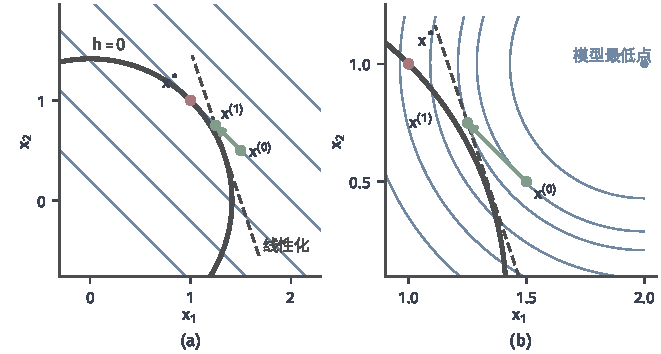
\includegraphics[width=112mm]{figures/05-optimization/06-constrained-optimization/matplotlib/sqp-circle-model/figure.pdf}
 \caption{问题~\eqref{eq:sqp-circle}的第一个局部模型。深灰粗线是圆$h=0$，虚线是线性化约束，绿点是迭代点，红点是解。(a)~蓝色直线是目标的等值线，步落在虚线上而不在圆上。(b)~放大的局部，蓝色圆是取$\bm{B}^{(0)}=2\bm{I}$时模型的等值线，模型无约束的最低点在右上方，受虚线限制后，最优步停在等值线与虚线相切的地方。}
 \label{fig:sqp-circle-model}
\end{BookInlineFigure}

\paragraph{目标怎样近似}
目标的一阶项仍取$\langle\nabla f(\bm{x}^{(t)}),\bm{d}\rangle$，二次项用一个对称矩阵$\bm{B}^{(t)}$。把两部分合起来，就得到局部模型。下面的定义里$\bm{B}^{(t)}$暂时留作待定，它的选取马上讨论。

\begin{definition}[局部二次规划与SQP]
\label{def:sqp-subproblem}
给定当前点$\bm{x}^{(t)}$与对称矩阵$\bm{B}^{(t)}$，\term{局部二次规划}（local quadratic program）是以$\bm{d}\in\mathbb{R}^n$为未知量的问题
\begin{equation}
 \begin{aligned}
 \min_{\bm{d}}\quad & \langle\nabla f(\bm{x}^{(t)}),\bm{d}\rangle+\frac12\bm{d}^\top\bm{B}^{(t)}\bm{d}\\
 \text{s.t.}\quad & \bm{h}^{(t)}+\bm{A}^{(t)}\bm{d}=\bm{0},\\
 & \bm{g}^{(t)}+\bm{G}^{(t)}\bm{d}\leq\bm{0}.
 \end{aligned}
 \label{eq:sqp-qp}
\end{equation}
反复构造并求解这样的子问题、用其解更新迭代点和乘子的方法，称为\term{序列二次规划}（sequential quadratic programming，SQP）。
\end{definition}

目标是二次的、约束是线性的，这就是第~\ref{chap:quadratic-conic-programming}章的二次规划（QP）。每一项的职责不同：目标梯度指出一阶意义下该往哪里走；$\bm{h}^{(t)},\bm{g}^{(t)}$说明当前违约多少；两个Jacobian说明约束怎样随步变化；$\bm{B}^{(t)}$说明走远了之后模型该怎样弯曲。

\paragraph{曲率为什么不能只取目标的Hessian}
最自然的想法是令$\bm{B}^{(t)}=\nabla^2f(\bm{x}^{(t)})$。式~\eqref{eq:sqp-circle}直接否定了这个想法。这里$\nabla^2f=\bm{0}$，模型的目标退化成线性函数，而可行集是一条直线，只要目标沿这条直线的斜率不为零，模型就没有下界。可是真实问题在圆上明明有一个弯曲的碗。

这只碗来自约束的弯曲。设想沿圆周走：坐标$x_1,x_2$本身在转弯，所以线性函数$f$沿圆周读出来的数值是弯的。模型把圆拉直成了直线，这部分弯曲必须另外算回目标的二次项。

下面把这件事算清楚。设$\bm{x}(s)$是一条留在等式约束上的光滑曲线，它在$s=0$处经过$\bm{x}$，速度是$\bm{v}$，加速度是$\bm{w}$。对恒等式$h_j(\bm{x}(s))=0$在$s=0$处求两次导数，得到
\[
 \langle\nabla h_j(\bm{x}),\bm{v}\rangle=0,\qquad
 \langle\nabla h_j(\bm{x}),\bm{w}\rangle+\bm{v}^\top\nabla^2h_j(\bm{x})\bm{v}=0.
\]

目标沿这条曲线的二阶导数由链式法则给出，它含有加速度$\bm{w}$：
\[
 \frac{\mathrm{d}^2}{\mathrm{d}s^2}f(\bm{x}(s))\Big|_{s=0}
 =\bm{v}^\top\nabla^2f(\bm{x})\bm{v}+\langle\nabla f(\bm{x}),\bm{w}\rangle.
\]

第~\ref{chap:constrained-optimality}章的一阶条件说，KKT点上$\nabla f+\sum_j\nu_j\nabla h_j=\bm{0}$，这里记Lagrange函数为$\mathcal{L}=f+\sum_i\lambda_ig_i+\sum_j\nu_jh_j$。把$\nabla f$代换掉，再用前面关于$\bm{w}$的恒等式，得到
\[
 \langle\nabla f,\bm{w}\rangle=-\sum_j\nu_j\langle\nabla h_j,\bm{w}\rangle=\sum_j\nu_j\bm{v}^\top\nabla^2h_j\bm{v}.
\]

代回上式，加速度消失了，剩下的正是Lagrange函数的Hessian：
\begin{equation}
 \frac{\mathrm{d}^2}{\mathrm{d}s^2}f(\bm{x}(s))\Big|_{s=0}
 =\bm{v}^\top\nabla^2_{\bm{x}\bm{x}}\mathcal{L}(\bm{x},\bm{\nu})\bm{v}.
 \label{eq:sqp-curve-curvature}
\end{equation}
这里乘子把约束的弯曲折算成了目标的弯曲，它正是第~\ref{chap:constrained-optimality}章二阶条件里出现$\nabla^2_{\bm{x}\bm{x}}\mathcal{L}$的原因。活动的不等式在其边界上同样处理，不活动的不等式乘子为零，不贡献曲率。

在圆上验证一下。沿圆取弧长参数$s$，解$\bm{x}^\star$处的乘子由$(-1,-1)^\top+\nu(2,2)^\top=\bm{0}$得$\nu^\star=1/2$，于是
\[
 \nabla^2_{\bm{x}\bm{x}}\mathcal{L}=2\nu^\star\bm{I}=\bm{I}.
\]

单位切向量$\bm{v}$给出$\bm{v}^\top\bm{I}\bm{v}=1$。另一方面，沿圆有$f=-2\cos(s/\sqrt2)$，它在$s=0$处的二阶导数是
\[
 \frac{\mathrm{d}^2f}{\mathrm{d}s^2}\Big|_{s=0}=2\cdot\frac12=1,
\]
两者相等。图~\ref{fig:sqp-curvature-circle}(a)画的就是这件事：带Lagrange曲率的模型与圆上的目标贴合，只用$\nabla^2f$的模型是一条平线。

\begin{BookInlineFigure}
 \centering
 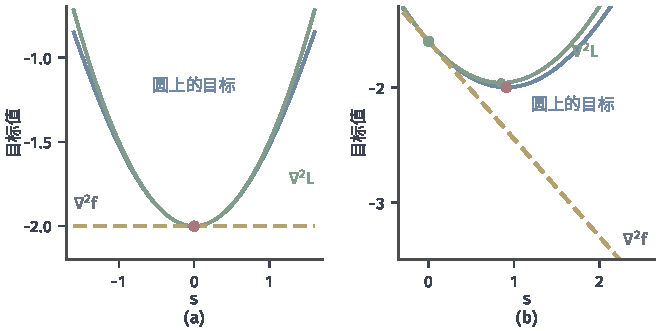
\includegraphics[width=112mm]{figures/05-optimization/06-constrained-optimization/matplotlib/sqp-curvature-along-circle/figure.pdf}
 \caption{沿约束的目标与两种模型，$s$是弧长（对模型是沿切线的距离）。蓝线是圆上真实的目标；绿线的二次项取$\nabla^2_{\bm{x}\bm{x}}\mathcal{L}=\bm{I}$；黄色虚线的二次项取$\nabla^2f=\bm{0}$。(a)~在解$\bm{x}^\star$处（红点）。(b)~在圆上的点$(1.4,0.2)^\top$处（左侧绿点）：绿色模型的最低点靠近真实最低点，只用$\nabla^2f$的模型沿切线一路下降，没有下界。}
 \label{fig:sqp-curvature-circle}
\end{BookInlineFigure}

式~\eqref{eq:sqp-curve-curvature}的推导用到了KKT点上的梯度关系，所以严格说它是解处的性质。迭代中手里只有估计值，于是取
\begin{equation}
 \bm{B}^{(t)}=\nabla^2_{\bm{x}\bm{x}}\mathcal{L}(\bm{x}^{(t)},\bm{\lambda}^{(t)},\bm{\nu}^{(t)})
 =\nabla^2f+\sum_{i=1}^m\lambda_i^{(t)}\nabla^2g_i+\sum_{j=1}^p\nu_j^{(t)}\nabla^2h_j,
 \label{eq:sqp-lagrangian-hessian}
\end{equation}
右端都在$\bm{x}^{(t)}$处取值，或取它的近似（第~\ref{sec:sqp-quasi-newton}节）。这解释了SQP为什么要同时维护原始变量和乘子：没有乘子，就写不出模型的曲率。

图~\ref{fig:sqp-curvature-circle}(b)显示了乘子估计不太准时的情形。点$(1.4,0.2)^\top$在圆上但不是解，取$\nu=1/2$，绿色模型的最低点仍然靠近真实的最低点。类比“局部模型信多远”：线性化约束告诉我们该待在哪里，乘子曲率告诉我们沿着允许的方向能走多远。这个类比在远离解时失效，那时乘子可能是错的，模型未必是碗，这是第~\ref{sec:sqp-curvature}节的话题。

\paragraph{子问题的乘子}
QP也有自己的乘子。记不等式的乘子为$\hat{\bm{\lambda}}$，等式的乘子为$\hat{\bm{\nu}}$。线性约束本身满足约束资格，所以把第~\ref{chap:constrained-optimality}章的KKT条件用于式~\eqref{eq:sqp-qp}时，它的每个局部解都满足
\begin{equation}
 \begin{gathered}
 \bm{B}^{(t)}\bm{d}+\nabla f(\bm{x}^{(t)})+(\bm{A}^{(t)})^\top\hat{\bm{\nu}}+(\bm{G}^{(t)})^\top\hat{\bm{\lambda}}=\bm{0},\\
 \bm{h}^{(t)}+\bm{A}^{(t)}\bm{d}=\bm{0},\qquad \bm{g}^{(t)}+\bm{G}^{(t)}\bm{d}\leq\bm{0},\\
 \hat{\bm{\lambda}}\geq\bm{0},\qquad \hat\lambda_i\bigl(g_i^{(t)}+\langle\nabla g_i^{(t)},\bm{d}\rangle\bigr)=0,\quad i=1,\ldots,m.
 \end{gathered}
 \label{eq:sqp-qp-kkt}
\end{equation}

把$\bm{d}=\bm{0}$代入式~\eqref{eq:sqp-qp-kkt}，第一行成为原问题的Lagrange驻定条件，第二行成为原问题的可行性，第三行成为原问题的乘子非负与互补。这就是下面的引理，它说明模型和原问题在解处是一致的。

\begin{lemma}[零步与KKT点]
\label{lem:sqp-zero-step}
$\bm{d}=\bm{0}$连同乘子$(\hat{\bm{\lambda}},\hat{\bm{\nu}})$满足式~\eqref{eq:sqp-qp-kkt}，当且仅当$(\bm{x}^{(t)},\hat{\bm{\lambda}},\hat{\bm{\nu}})$满足原问题~\eqref{eq:sqp-nlp}的KKT条件。
\end{lemma}

\begin{proof}
令$\bm{d}=\bm{0}$，含$\bm{B}^{(t)}$的项消失，线性化项都等于在$\bm{x}^{(t)}$处的取值。式~\eqref{eq:sqp-qp-kkt}逐行就是原问题在$\bm{x}^{(t)}$处的驻定、可行、乘子非负和互补条件，反过来也一样。
\end{proof}

引理与$\bm{B}^{(t)}$无关，所以不论曲率怎样近似，模型的不动点都是原问题的KKT点。曲率只影响走向这个点的速度。解完QP后，新的乘子估计可以直接取子问题的乘子，当步长$\alpha^{(t)}\in(0,1]$时按比例插值：
\begin{equation}
 \begin{aligned}
 \bm{\lambda}^{(t+1)}&=\bm{\lambda}^{(t)}+\alpha^{(t)}\bigl(\hat{\bm{\lambda}}-\bm{\lambda}^{(t)}\bigr),\\
 \bm{\nu}^{(t+1)}&=\bm{\nu}^{(t)}+\alpha^{(t)}\bigl(\hat{\bm{\nu}}-\bm{\nu}^{(t)}\bigr).
 \end{aligned}
 \label{eq:sqp-multiplier-update}
\end{equation}

\paragraph{一轮计算的结构}
图~\ref{fig:sqp-loop}把一轮计算的部件排在一起。求值之后得到子问题，子问题给出步和乘子，步还要放回原问题检验。两处可能出岔：子问题可能无解，步也可能被拒绝。后面各节依次处理这些部件。

\begin{BookInlineFigure}
 \centering
 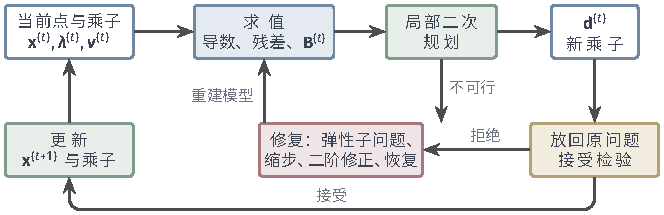
\includegraphics[width=112mm]{figures/05-optimization/06-constrained-optimization/tikz/sqp-loop/figure.pdf}
 \caption{SQP一轮计算的结构。绿框是模型的构造与接受后的更新，黄框是把步放回非线性问题的检验，红框是子问题无解或候选步被拒绝时的修复。修复之后重新建模或重新求解。}
 \label{fig:sqp-loop}
\end{BookInlineFigure}

需要说明的是，SQP规定的是“解一列局部QP”，并没有规定用什么方法解QP。下面用有效集法讲解，因为它的逻辑最贴近“哪些约束算数”这个问题；QP也可以用内点法或其他方法求解，第~\ref{chap:nonlinear-interior-point}章的内点法思想同样适用于QP。

局部模型还有一点要记住：模型可行不等于原问题可行。式~\eqref{eq:sqp-linearized}只是切平面，步$\bm{d}$落在切平面上，一般不在原来的曲面上。这个缺口贯穿全章，第~\ref{sec:sqp-acceptance}节和第~\ref{sec:sqp-repair}节专门处理它。
